\documentclass{article}

\PassOptionsToPackage{numbers,compress}{natbib}
\usepackage[final]{nips_2017}


%--------------Document configuration begins--------------
\usepackage{amsthm}
\usepackage[colorlinks]{hyperref}
\usepackage[capitalise]{cleveref}
%--------------Document configuration ends--------------

%Theorems, lemmas, proofs, etc
\theoremstyle{plain}
\newtheorem{theorem}{Theorem}[section]
\newtheorem{proposition}[theorem]{Proposition}
\newtheorem{lemma}[theorem]{Lemma}
\theoremstyle{definition}
\newtheorem{definition}[theorem]{Definition}
\newtheorem{remark}[theorem]{Remark}
\newtheorem{corollary}[theorem]{Corollary}
\renewcommand{\proofname}{{\sc Proof}}


%Import personal commands 
\usepackage{commandscsp}

\title{Computing Constrained Shortest-Paths at Scale}
\author{}

\begin{document}

\maketitle

\begin{abstract}
	Motivated by the needs of modern transportation service platforms, we study the problem of computing constrained shortest paths (CSP) at scale via preprocessing and network augmentation techniques.
Our work makes two contributions in this regard:\\
1. We propose a scalable algorithm for CSP queries, and show how its performance can be parametrized in terms of a new network primitive, the \emph{constrained highway dimension}. 
This development is analogous to recent work which established the \emph{highway dimension} as the appropriate primitive for characterizing the performance of existing shortest-path (SP) algorithms. 
Our main theoretical contribution is deriving conditions relating the two notions, thereby providing a characterization of networks where CSP and SP queries are of comparable hardness.\\
2. We develop practical algorithms for scalable CSP computation, augmenting our theory with additional network clustering heuristics. 
We evaluate these algorithms on real-world datasets to validate our theoretical findings. 
Our techniques are orders of magnitude faster than existing approaches, while requiring only limited additional storage and preprocessing.
\end{abstract}

\section{Introduction}
% !TEX root = main_nips.tex
We consider the fast computation of constrained shortest paths in large-scale graphs, using preprocessing and graph augmentation techniques.
The Shortest-path (SP) problem is one of the canonical algorithm design problems.
In recent years, however, it has been revolutionized both in terms of academic research as well as real-world applications (cf.~\cite{goldberg_survey,dimacs09} for surveys).
In particular, the use of preprocessing techniques and network augmentation has led to dramatic improvements in the speed and scalability of SP computation in road networks.
These techniques however do not extend to constrained shortest-path (CSP) problems, and our work aims to bridge this gap.

The SP and CSP problems can be summarized as follows: We are given a graph $G$, where each edge has an associated \emph{length} and \emph{cost}. 
Now, given any two nodes $s,t$, the SP problem requires finding an  $s\rightarrow t$ path of minimum length; the CSP problem takes in a further input of a budget $b$, and requires finding a minimum length $s\rightarrow t$ path \emph{which moreover has a total cost less than $b$}.
The two problems, though similar, have very different basic complexity: SP computation admits a polynomial-time algorithm (in particular, the famous Dijkstra's algorithm), while the problem of CSP computation is known to be NP-Hard~\cite{csp_survey}.
That said, a standard dynamic programming approach allows CSP computation in pseudo-polynomial time when the costs are discrete (in particular, polynomial in the maximum budget), and also admits a natural scaling-based FPTAS for continuous costs (akin to the knapsack FPTAS).

Although there is a rich literature on CSP problems (cf. \cite{csp_survey} for a survey), there is little work on studying ways of using preprocessing and graph augmentation to speed up CSP computation. Our work here aims to address this gap, motivated by the success of similar approaches for SP computation. Moreover, we believe that there is a need for such techniques in several modern applications, as we discuss next. 


\paragraph*{Applications of large-scale CSP computation}

Our interest in CSP computation is motivated primarily by the requirements of transportation platforms like Lyft, Uber, Waze etc., for accurate routing and travel-time estimates with probabilistic guarantees.
Fast routing and trip-time estimation, driven by fast SP engines (for example, OSRM~\cite{OSRM}), have provided impetus to the increasing use of mobile maps.
These techniques however do not make full use of available real-time traffic information; in particular, SP queries are unable to incorporate uncertainties in travel times, and hence often give inaccurate trip-time estimates in settings with high traffic uncertainty.


A natural way to incorporate travel-time uncertainty is to compute the shortest path subject to a reliability constraint.
In particular, in many settings, we want \emph{robust} travel time estimates: formally, we require that given $s,t$ and parameters $p,\delta$, a routing algorithm returns an $(s,t)$-path $P$ minimizing $\E[\ell(P)]$, subject to $\Pr[\ell(P)>\E[\ell(P)]+\delta]\leq p$.
Even assuming that travel times on different road segments are independent, computing this exactly for general distributions is expensive due to the need for computing convolutions of distributions. However, for uncorrelated travel-times, we have $\Pr[\sum_eT_e>\E[\sum_eT_e])+\delta]\leq \sum_e\Var(T_e)/\delta^2$ by Chebyshev's inequality; using this, we can replace the robust trip-time estimation problem with the following
\begin{center}
$\min_{ P\in\Pst}\sum_{i\in P}\mu_i \qquad \mbox{s.t.}\qquad \sum_{i\in P}\sigma^2_i\leq \delta^2p.$
\end{center}
This is now a CSP problem. Note that the solution, though not necessarily optimal, always respects the reliability constraint -- this is often more critical for practical applications.


Another problem that can be modeled as a CSP is that of finding \emph{reliable shortest paths}.
Consider the case where each edge has a probability $q_e$ of triggering a bad event, with resulting penalty $p$ (for example, slowdowns due to accidents).
In this case, we want to minimize the travel time as well as the expected penalty.
In this case, assuming independence, we have the following natural problem
\begin{center}
$\min_{P\in\Pst} \ell(P)+p\prn*{1-\prod_{e\in P}(1-q_e)}.$
\end{center}
This model is considered in \cite{fareevasion} (for routing with fare evasion, where $q_e$ is the probability of encountering an inspector, and $p$ the penalty), where the authors suggest using a CSP formulation, wherein the non-linear objective is replaced by a linear constraint by taking logarithms.

%Finally, another class of problems which is related to the CSP is that of routing under \emph{label constraints} \cite{language_csp,rice_csp}, wherein we want shortest routes which satisfy certain properties (for example, those that avoid toll roads). The main idea in such problems (as in the CSP) is to use an appropriate augmented graph that converts feasible shortest paths to shortest paths. Our results extend to these applications as well.

\subsection{Our Contributions}

\noindent We aim to address the following overarching questions:
\begin{enumerate}[nosep,leftmargin=*]
\item How can we use preprocessing and graph augmentation techniques to speed up CSP computation. 
\item How can we give preprocessing/storage/query time guarantees for such techniques.
\end{enumerate}

For the SP problem, there was significant initial development on the first question, leading to many different techniques~\cite{dimacs09}, which worked well in practice, but had no performance guarantees.
Abraham et al.~\cite{highway2013, highway2010} then proposed the \emph{Highway Dimension} (HD), a graph structural metric, which they showed could parametrize the preprocessing, storage and query time of several of these heuristics (hub labels, contraction hierarchies, etc.).
Our work adopts a similar program; in particular, our contributions are as follows:
\begin{itemize}[nosep,leftmargin=*]
\item \textbf{Theoretical contributions}: 
We extend the HD to directed graphs and general path systems (Section~\ref{ssec:hddef}), and define an analogous notion of a \emph{constrained highway dimension} (CHD) for Pareto efficient paths (Section~\ref{sec:chd}). We then construct an augmented graph (Section~\ref{ssec:aug}) under which efficient paths are mapped to shortest paths, and use it to develop hub labels for CSP queries, whose complexity is parameterized by the CHD (Section~\ref{ssec:hlcsp}).
Finally, we show that although the CHD can be much bigger than the HD in general, the two can be related under an additional \emph{partial witness condition} (Section~\ref{ssec:hdvschd}). This provides some justification for the use of preprocessing techniques for CSP, as it suggests that they should work well in settings where SP computation admits good speedup techniques.
\item \textbf{Practical contributions}: Although the theoretical results justify the use of preprocessing techniques for CSP, they are impractical for real networks. We show how we can adapt our theoretical ideas to develop a practical construction technique for hub labels that support CSP queries (Section~\ref{sec:numeric}). We then evaluate our algorithm on datasets with detailed travel-time information for San Francisco and Luxembourg (Section~\ref{sec:exp}). Our experiments show that our hub labels support query times which are orders of magnitude faster than existing techniques (without preprocessing), have small per-node storage requirements, and good preprocessing times even on a single machine. 
\end{itemize}	

\subsection{Related work}

As we mention before, our work is inspired by the recent developments (both theoretical and practical) in shortest path algorithms~\cite{highway2013,hubimplem,highway2010,dimacs09,geisberger_ch_definition,skeleton}; refer~\cite{goldberg_survey} for an excellent survey of these developments. 


The problem of finding robust shortest paths is closely related to the stochastic on-time arrival (SOTA) problem~\cite{fan2005arriving}.
The SOTA problem with Gaussian travel times was solved via exhaustive search~\cite{nikolova_gaussian}. The optimal policy under discrete distributions was given in~\cite{samaranayake2012speedup}, and pre-processing policies were considered in~\cite{sabran2014precomputation}. Finally, ~\cite{nikolova_discretization} provides an approximation technique based on discretization for DAGs.

The primary speedup technique we use in our work is that of hub labels (HL). This was introduced first in~\cite{cohen_definition_hl}. More recently, HL was shown to admit the best query time bounds in low HD graphs~\cite{highway2013,highway2010}, and this observation was experimentally confirmed in~\cite{hubimplem} (see also Figure 7 in~\cite{goldberg_survey}).  
Finally, the HD-based bounds for hub labels was shown to be tight in~\cite{babenko_hl_complexity,white_complexity_hd}, and it was also shown that finding optimal hub labels is NP hard.

There is an extensive literature on CSP problems, which is well surveyed in~\cite{csp_survey}; most of this work however considers only query-time techniques without preprocessing. Our graph augmentation technique is similar to that proposed in~\cite{alex_bicriteria}, which is based on a dynamic programming approach. 

Finally, a related class of problems to CSP is that of shortest paths under label constraints, first introduced in~\cite{language_csp}. Contraction hierarchies were adapted to solve a restricted class of such problems in~\cite{rice_csp}, where the aim was to find shortest paths that avoided certain labels (for example, toll roads/ferries). Our work is similar in spirit to this paper. Note however that the label-constrained problem in~\cite{rice_csp} is a concatenation of parallel shortest-path problems, and involves only local constraints. 
In contrast, the CSP is NP-hard as it involves global constraints on paths; consequently, a small number of edges with costs can affect all nodes. Thus, though the techniques in~\cite{rice_csp} do not apply to our setting, our theoretical results do in fact shed light on why contraction hierarchies work well in their setting.
%%!TEX root = main_vldb.tex
We consider the problem of fast computation of constrained shortest paths in large-scale graphs, using preprocessing and graph augmentation techniques.
The Shortest-path (SP) problem is one of the canonical algorithm design problems.
In recent years, however, it has been revolutionized both in terms of academic research as well as real-world applications (cf.~\cite{goldberg_survey,dimacs09} for surveys).
In particular, the use of preprocessing techniques and network augmentation has led to dramatic improvements in the speed and scalability of SP computation in road networks.
These techniques however do not extend to constrained shortest-path (CSP) problems, and our work aims to bridge this gap.

The SP and CSP problems can be summarized as follows: We are given a graph $G$, where each edge has an associated \emph{length} and \emph{cost}. 
Now, given any two nodes $s,t$, the SP problem requires finding an  $s\rightarrow t$ path of minimum length; the CSP problem takes in a further input of a budget $b$, and requires finding a minimum length $s\rightarrow t$ path \emph{which moreover has a total cost less than $b$}.
The two problems, though similar, have very different basic complexity: SP computation admits a polynomial-time algorithm (in particular, the famous Dijkstra's algorithm), while the problem of CSP computation is known to be NP-Hard~\cite{csp_survey}.
That said, a standard dynamic programming approach allows CSP computation in pseudo-polynomial time when the costs are discrete (in particular, polynomial in the maximum budget), and also admits a natural scaling-based FPTAS for continuous costs (akin to the knapsack FPTAS).

Although there is a rich literature on CSP problems (cf. \cite{csp_survey} for a survey), there is little work on studying ways of using preprocessing and graph augmentation to speed up CSP computation. Our work here aims to address this gap, motivated by the success of similar approaches for SP computation. Moreover, we believe that there is a need for such techniques in several modern applications, as we discuss next. 


\paragraph*{Applications of large-scale CSP computation}

Our interest in CSP computation is motivated primarily by the requirements of transportation platforms like Lyft, Uber, Waze etc., for accurate routing and travel-time estimates with probabilistic guarantees.
Fast routing and trip-time estimation, driven by fast SP engines (for example, OSRM~\cite{OSRM}), have provided impetus to the increasing use of mobile maps.
These techniques however do not make full use of available real-time traffic information; in particular, SP queries are unable to incorporate uncertainties in travel times, and hence often give inaccurate trip-time estimates in settings with high traffic uncertainty.


A natural way to incorporate travel-time uncertainty is to compute the shortest path subject to a reliability constraint.
In particular, in many settings, we want \emph{robust} travel time estimates: formally, we require that given $s,t$ and parameters $p,\delta$, a routing algorithm returns an $(s,t)$-path $P$ minimizing $\E[\ell(P)]$, subject to $\Pr[\ell(P)>\E[\ell(P)]+\delta]\leq p$.
Even assuming that travel times on different road segments are independent, computing this exactly for general distributions is expensive due to the need for computing convolutions of distributions. However, for uncorrelated travel-times, we have $\Pr[\sum_eT_e>\E[\sum_eT_e])+\delta]\leq \sum_e\Var(T_e)/\delta^2$ by Chebyshev's inequality; using this, we can replace the robust trip-time estimation problem with the following
\[
\min_{ P\in\calP_{s,t}}\sum_{i\in P}\mu_i \qquad \text{s.t.}\qquad \sum_{i\in P}\sigma^2_i\leq \delta^2p.
\]
This is now a CSP problem. Note that the solution, though not necessarily optimal, always respects the reliability constraint -- this is often more critical for practical applications.


Another natural problem that can be modeled as a CSP is that of finding shortest paths satisfying some \emph{reliability constraint}.
Consider the case where each edge has a probability $q_e$ of triggering a bad event, with resulting penalty $p$ (for example, slowdowns due to accidents).
In this case, we want to minimize the travel time as well as the expected penalty.
In this case, assuming independence, we have the following natural problem
\[
\min_{P\in\calP_{s,t}} \ell(P)+p\Bigl(1-\prod_{e\in P}(1-q_e)\Bigr).
\]
This model is considered in \citet{fareevasion} (for routing with fare evasion, where $q_e$ is the probability of encountering an inspector, and $p$ the penalty), where the authors suggest using a CSP formulation, wherein the non-linear objective is replaced by a linear constraint by taking logarithms.

Finally, another class of problems which is related to the CSP is that of routing under \emph{label constraints} \cite{language_csp,rice_csp}, wherein we want shortest routes which satisfy certain properties (for example, those that avoid toll roads). Although different in formulation, the main idea in such problems, as in the CSP, is to use an appropriate augmented graph that converts feasible shortest paths to shortest paths. Our results extend to these applications as well.

\subsection{Our Contributions}

\noindent There are two natural questions re fast CSP computation:
\begin{enumerate}[nosep,leftmargin=*]
\item How can we use preprocessing and graph augmentation techniques to speed up CSP computation 
\item How can we give preprocessing/storage/query time guarantees for such techniques
\end{enumerate}
The concept of Highway Dimension (HD) \cite{highway2010,highway2013} allows to prove the efficiency of shortest path computations in undirected graphs.
We will see that directed graphs are fundamental for the analysis of constrained paths.
As a first step, we extend the notions of HD to directed graphs.

\sbnote{copied from abstract}
Our work extends these ideas to CSP queries, via two main contributions:  \todo{add references to results here}
\begin{itemize}[nosep,leftmargin=*]
	\item Theoretical contributions: We adapt existing preprocessing techniques for fast SP queries (hub labels and contraction hierarchies) to handle CSP queries. More importantly, we extend the idea of \emph{highway-dimension}, a proposed measure of the complexity of SP speedup techniques, to an analogous \emph{constrained highway dimension} for CSP queries.
	We also show that the two notions can be related under an additional partial witness condition, which we argue is natural for road networks.
	\item Practical contributions: We develop a practical algorithm for fast CSP queries, which combines the hub labels technique for SP computations with an augmented graph that encodes efficient paths for the CSP problem. We evaluate our algorithm on datasets with detailed travel-time information for San Francisco and Luxembourg, and show that our algorithms support query times which are orders of magnitude than existing techniques (without preprocessing), have small per-node storage requirements, and good preprocessing times even on a single machine. 
\end{itemize}	


\subsection{Related work}

Bicriteria with augmented graph and robot applications \cite{alex_bicriteria}

Introduced hub labels\cite{cohen_definition_hl}

Survey on shortest path algorithms \cite{goldberg_survey}

Bounds for hub labels in different classes of graphs. 
Show that there exists a hierarchichal hub label meeting the bound of HD \cite{babenko_hl_complexity}

Shows that the lower bounds of the HL size, given by the HD, is tight for a family of graphs \cite{white_complexity_hd}

Introduce a class of restrictions as label constraints \cite{language_csp}

For a restricted language, it is possible to use CH for the problem \cite{rice_csp}

Skeleton dimension \cite{skeleton}

Survey on CSP \cite{csp_survey}

This objective is closely related to the stochastic on time arrival (SOTA) problem \cite{fan2005arriving}.

SOTA problem with gaussian travel times solved by exhaustive search \cite{nikolova_gaussian}, optimal policy \cite{samaranayake2012speedup}, pre-processing \cite{sabran2014precomputation} anb solved with discretization for directed acyclic graphs \cite{nikolova_discretization}

\section{Preliminaries}
\label{sec:prelim}

\subsection{Basic Setting}
\label{ssec:basic}
We consider a directed graph $G=(V,E)$, where each edge $e\in E$ has an associated \emph{length} $\ell(e)\in\N_+$, and \emph{cost} $c(e)\in\N_+\cup\crl{0}$.
The triplet $(G,\ell,c)$ is called a \emph{network}.
For any path $P$, we define its length $\ell(P)$ and cost $c(P)$ as the sum of edge lengths and edge costs in $P$. 
Our goal is to develop a data structure to answer \emph{Constrained Shortest-Path} (CSP) queries efficiently as described next.

\begin{problemdef}[framed]{Constrained Shortest-Path Queries}
	Input: & Graph $G=(V,E)$, costs $c$, lengths $\ell$, and maximum budget $B$.\\
	Preprocessing Task:& Create a data structure $\mathcal{S}$. \\
	Real Time Task:& For any source-terminal pair $s,t\in V$ and budget $b\leq B$, use $\mathcal{S}$ to return a path solving $\min\crl{\ell(P):c(P) \leq b, P \text{ is an } (s,t)\text{-path}}$.
	The triplet $(s,t,b)$ defines a \emph{query} and it is arbitrarily specified by the user. \\
  	Performance Metrics: &  Size of $\mathcal{S}$, preprocessing time (to compute $\mathcal{S}$), and query time (to return a path given $s,t,b$). 
\end{problemdef}


Note that the two computation times are in different scales.
Indeed, it is acceptable to have a preprocessing time of a few minutes, but the query time should be in milliseconds.
Observe also that the performance metrics are in conflict.
To illustrate this, define $n=\abs{V}$ as the number of nodes and consider two extreme cases.
(i) for each $(s,t,b)$ we store in $\mathcal{S}$ the solution to the associated query, which has $O(1)$ query time, but space $\abs{\mathcal{S}}=\Omega(Bn^2)$.
(ii) use no data structure, which consumes no space, but requires $\Omega(bn\log n)$ query time using Dijkstra (see \cref{prop:shorteffic}).

We stress that either storage $\Omega(n^2)$ or query time $\Omega(n)$ is unacceptable for modern applications.
The goal is to find $\mathcal{S}$ in polynomial time with small storage and fast query time.

\medskip
\paragraph{Our Results.}
We identify a parameter $\hc$, called the Constrained Highway Dimension (CHD), which generalizes the concept introduced in \citep{hd_journal}, and obtain the results below.
In each case, the data structure can be computed in polynomial time.
$D$ represents the diameter of the graph.
\begin{enumerate}
\item We give a data structure of size $\tilde O(nB\cdot B\hc\log D)$ and query time $\tilde O(b\hc\log D)$ for any $(s,t,b)$, see \cref{theo:HLeff,thm:markedhubs}.
We relate $\hc$ to the HD in \cref{theo:witness_doubling}.
\item We introduce the notion of \emph{Average CHD}, which is strictly weaker than CHD, and show that we can obtain a data structure with the same guarantees, but the query time is in average over $(s,t)$, see \cref{theo:preproc_avg}.
\item Building on the average CHD, we give a condition, interpreted as having few overpasses, such that the query time is  $\tilde O(bh\alpha\log D)$, average over $(s,t)$, with space requirement $\tilde O(n B\cdot Bh\alpha\log D)$, where $h$ is the HD and $\alpha$ the doubling constant, see \cref{theo:overpasses}.
We observe that, for road networks, it is conjectured that $h=\text{polylog}(n)$ and $\alpha=O(1)$, hence our result explains the good empirical performance of our algorithm, see \cref{sec:numeric}.
\end{enumerate}


\medskip
\paragraph{Final Setup Details.}
For any source-terminal pair $s,t\in V$, we denote by $\Pst$ the set of all simple $(s,t)$-paths (without loops or cycles). 
Throughout this work, we only consider simple paths, which we refer to as paths for brevity.
We denote the shortest $(s,t)$-path (if it exists) as $P(s,t)$, and denote the set of all shortest paths in $G$ as $\PS$.

For each node $v$, we denote its degree $\Delta(v)$ as the sum of the in-degree and out-degree, and define the \emph{maximum degree} $\Delta \defeq \max_v\Delta(v)$.
For $s,t\in V$, the distance from $s$ to $t$, denoted $\dist(s,t)$, is the smallest length among all paths $P\in\Pst$.
We define $\dist(s,t|b)$ to be the length of the shortest path with cost at most $b$, i.e., the length of the path returned by the query $(s,t,b)$.
If there is no feasible solution, we define $\dist(s,t|b)=\infty$.

For a node $v$ and a path $P$, we abuse notation to denote $\dist(v,P)$ as the minimum distance from $v$ to any node $w\in P$; the distance $\dist(P,v)$ from $P$ to $v$ is defined analogously.
Note that  $\dist(P,v)$ and  $\dist(v,P)$ need not be the same as the graph is directed.
We define $D\defeq\max_{P\in\PS}\ell(P)$ to be the diameter of $G$.


For $r>0$ and $v\in V$, we define the \emph{forward and reverse balls of radius $r$} by $\Bf_r(v)\defeq\{u\in V: \dist(v,u)\leq r\}$ and $\Bb_r(v)\defeq\{u\in V: \dist(u,v)\leq r\}$, and also define $B_r(v)\defeq\Bf_r(v)\cup\Bb_r(v)$.
Finally, a graph $G$ is said to have a \emph{doubling constant} $\alpha$ if, for any node $v$ and any $r>0$, the ball $B_{2r}(v)$ can be covered by at most $\alpha$ balls of radius $r$.

\subsection{Hitting sets and the highway dimension}
\label{ssec:hddef}
We now define some additional network primitives, which we need to parametrize the performance of our CSP algorithms. 
In particular, we use the \emph{highway dimension}, introduced by Abraham et al.~\cite{highway2013,highway2010} to parametrize shortest-path computations in undirected graphs. As a first step, we need to extend the definitions to directed graphs and to general sets of paths, not necessarily shortest.


We define a \emph{path system} $\calQ$ as any collection of paths.
We say that a set $C\subseteq V$ \emph{hits} any given path $Q$ if some node in $Q$ belongs to $C$. Moreover, we say that $C$ is a \emph{hitting set for a path system} $\calQ$ if it hits every $Q\in\calQ$. 
For any $r>0$, we say a path $Q$ is $r$-significant if $\ell(Q)>r$. 
For a given path system $\calQ$, we denote $\calQ_r$ as the set of all $r$-significant paths in $\calQ$.
Hitting sets are measured with respect to the sparsity and the ability to hit significant paths, formally we desire the following.
%Hitting sets are useful for compressing path systems. In particular, even if the hitting set is large, the extent to which a path system can be compressed depends on the \emph{local sparsity} of hitting sets with respect to \emph{significant paths} of $\calQ$.

\begin{definition}[Locally-Sparse Hitting Sets]\label{def:lshs}
Given a path system $\calQ$ and $r>0$, an $(h,r)$ locally-sparse hitting set (or $(h,r)$-LSHS) is a set $C\subseteq V$ with two properties: 
\begin{enumerate}[nosep]
\item Hitting: $C$ is a hitting set for $\calQ_r$.
\item Local sparsity: for every $v\in V$, $\abs*{B_{2r}(v)\cap C}\leq h$.
\end{enumerate}
\end{definition}


As we discuss in \cref{ssec:hldef}, the existence of $(h,r)$-LSHS immediately enables the compression of path system $\calQ$ via the construction of \emph{hub labels}. 
However, the existence of LSHS does not guarantee the ability to efficiently compute these objects. 
To address this, it was shown that the \emph{highway dimension} is a property that ensures both existence and efficient computation of LSHS \cite{highway2013}. 
To define the highway dimension, we first need two additional definitions:
for $v\in V, r>0$, we define the \emph{forward and reverse path-neighborhoods} with respect to path system $\calQ$ as: $
S_r^+(v,\calQ) \defeq\crl*{Q\in\calQ_r: \dist(v,Q)\leq 2r}$ and  $S_r^-(v,\calQ) \defeq\crl*{Q\in\calQ_r: \dist(Q,v)\leq 2r}$.
As before, we have $S_r(v,\calQ) \defeq S_r^+(v,\calQ)\cup S_r^-(v,\calQ)$. Now we can define the highway dimension (HD) of a path system $\calQ$. Essentially, the HD re-orders the sequence of qualifiers in the definition of $(h,r)$-LSHS: it requires the existence of a small hitting set for each individual neighborhood, rather than a single hitting set which is locally sparse. 
\begin{definition}[Highway Dimension]	\label{def:hddef}
	A path system $\calQ$ has HD $h$ if, $\forall r>0,v\in V$, there exists a set $H_{v,r}\subseteq V$ such that $\card{H_{v,r}}\leq h$ and $H_{v,r}$ is a hitting set for $S_r(v,\calQ)$.
\end{definition}

The HD was defined in \cite{highway2013} for undirected graphs and the shortest-path system $\PS$; the above definition is the natural analog for directed graphs and general path systems.
As shorthand, we refer to the HD of $(G,\ell)$ as that of $\PS$. 
Note that $HD\leq h$ is a more stringent requirement than the existence of an $(h,r)$-LSHS $C$, since $C\cap B_{2r}(v)$ need not hit all the paths in $S_r(v,\calQ)$. 
However, if $G$ has $HD \leq h$, then this guarantees the existence of a $(h,r)$-LSHS.
\begin{proposition}\label{prop:equiv}
If the path system $\calQ$ has HD $h$, then, $\forall\,r>0$, there exists an $(h,r)$-LSHS.
\end{proposition}


This fact follows by adapting the proof from \cite[Theorem 4.2]{highway2013} to our general case.
More importantly, as we discuss in Section~\ref{sec:preproc}, if $G$ has $HD \leq h$, then this permits efficient computation of locally-sparse hitting sets.
In particular, for any $r$, a simple greedy algorithm gives an $(\Or(h\log n),r)$-LSHS, and a more complex algorithm (which is still poly-time) gives an $(\Or(h\Delta\log h\Delta),r)$-LSHS.
Finally, we briefly note that Definition~\ref{def:hddef} modifies the original definition of~\cite{highway2013} in two ways: $(i)$ we consider a less restrictive definition of path neighborhoods, that is appropriate for our needs, and $(ii)$ we generalize the notion to directed graphs and general path systems.
For $\PS$, a consequence of considering less-restrictive path-neighborhoods is that the highway dimension returned by our definition is smaller than that of \cite{highway2013}.
In particular, unlike \cite{highway2013}, the HD of $G$ as per our definition is not an upper bound to the maximum degree $\Delta$ or the doubling dimension $\alpha$.
We discuss the relation between the two definitions in detail in Appendix~\ref{app:generalhd}

\subsection{Shortest-Paths via Hub Labels}
\label{ssec:hldef}
Two of the most successful data-structures enabling fast shortest path queries at scale are \emph{contraction hierarchies} (CH)~\cite{geisberger_ch_definition} and \emph{hub labels} (HL)~\cite{cohen_definition_hl}.
These are general techniques which always guarantee correct SP computation, but have no uniform storage/query-time bounds for all graphs.
However, Abraham et al.~\cite{highway2013} show that for a graph with HD $\leq h$, the preprocessing time, storage requirements and query time of particular implementations of the CH and HL algorithms can be bounded solely in terms of $h$, the maximum degree $\Delta$ and the diameter $D$. 
We now explain the construction for HL for directed graphs; for the construction of CH see Appendix~\ref{sec:ch}.
HL was also shown to admit the best query-time guarantees in~\cite{highway2013}; consequently, we adapt the HL technique for scaling CSP computations in Section \ref{sec:chd}.

The basic HL technique is as follows:
Every node $v$ is associated with a \emph{hub labels}, $L(v) = \crl*{\Lf(v),\Lb(v)}$, comprising of a set of forward hubs $\Lf(v)$ and reverse hubs $\Lb(v)$.
We also store $\dist(v,w),\dist(u,v)$ for every $w\in\Lf(v),u\in\Lb(v)$.
The hub labels are said to satisfy the \emph{cover property} if, for any $s\neq t\in V$, $\Lf(s)\cap\Lb(t)$ contains at least one node in $P(s,t)$.
In the case that $t$ is not reachable from $s$, it must be that $\Lf(s)\cap\Lb(t)=\varnothing$.

With the aid of the cover property, we can obtain $\dist(s,t)$ by searching for the minimum value of $\dist(s,w)+\dist(w,t)$ over all nodes $w\in\Lf(s)\cap\Lb(t)$.
If the hubs are sorted by ID, this can be done in time $\Or(\card{\Lf(s)}+\card{\Lb(t)})$ via a single sweep.
Moreover, by storing the second node in $P(s,w)$ for each $w\in \Lf(s)$, and the second-last node in $P(w,t)$ for each $w\in \Lb(t)$, we can also recover the shortest path.
Now, each time we run a HL query, we find at least one new node $w\in P(s,t)$, $w\neq s,t$, is returned; we can then recurse to find subpaths $P(s,w)$ and $P(w,t)$.
Note that we need to store this extra information, as otherwise, we could have $\Lf(s)\cap\Lb(t)=\{s\}$.
Let $\Lm \defeq \max_v\abs*{L(v)}$ be the size of the maximum HL; then the per-node storage requirement is proportional to $\Lm$, while the query time is proportional to $\Lm\cdot P(s,t)$.

To construct hub labels with guarantees on preprocessing time and $\Lm$, we need the additional notion of a \emph{multi-scale LSHS}. 
For $i=1,\ldots,\log D$, we assume that graph $(G,\ell)$ admits a collection of sets $\crl*{C_i}$, such that each $C_i$ is an $(h,2^{i-1})$-LSHS.
Given such a collection $\crl*{C_i}$, we can now obtain small HL; we outline this construction for directed graphs, closely following the construction in \cite{highway2013} (Theorem 5.1) for the undirected case.
\begin{proposition}
\label{theo:construct_hl}
For $(G,\ell)$, given a multi-scale LSHS collection $\crl*{C_i;i=1,\ldots,\log D}$ (where each $C_i$ is an $(h,2^{i-1})$-LSHS), we can construct hub labels of size at most $h\log D$.
\end{proposition}
\begin{proof}
For each node $v$, we define the hub label $L(v)$ as
\begin{align*}
\Lf(v)\defeq  \bigcup_{i=1}^{\log D}C_i\cap \Bf_{2^i}(v)\;,\;
\Lb(v)\defeq \bigcup_{i=1}^{\log D}C_i\cap \Bb_{2^i}(v).
\end{align*}
Since each $C_i$ is an $(h,2^{i-1})$-LSHS which we intersect with balls of radius $2\cdot 2^{i-1}$, every set in the union contributes at most $h$ elements and the maximum size is as claimed.

To prove the cover property, we note that, if $t$ is not reachable from $s$, by definition $\Lf(s)\cap\Lb(t)=\varnothing$.
This is because the elements in $\Lf(s)$ are reachable from $s$ and the elements in $\Lb(t)$ reach $t$.
On the other hand, when $P(s,t)$ exists, let $i$ be such that $2^{i-1}<\ell(P(s,t))\leq 2^i$.
Now any point in the path belongs to both $\Bf_{2^i}(s)$ and $\Bb_{2^i}(t)$, and hence $C_i\cap P(s,t)$  (which is not empty since $C_i$ hits all SP of length $\geq 2^{i-1}$) is then in both hubs, which shows the result.
\end{proof}


Finally, we need to compute the desired multi-scale LSHS in polynomial time.
As we mention before, a greedy algorithm returns a $\Or(h\log n)$ approximation to any $(h,r)$-LSHS; however if the HD $\leq h$, this can be improved to obtain a $\Or(h\Delta\log(h\Delta))$ approximation; this argument, which extends Corollary 7.3 in \cite{highway2013}, is presented in Section~\ref{sec:preproc}.
A more subtle point is that the resulting algorithm, even though admitting a polynomial time guarantee, is impractical for large networks; in Section~\ref{sec:numeric}, we discuss heuristics that work better in practice.

\section{Scalable CSP Algorithms:\texorpdfstring{\\}{ } Theoretical Guarantees}
\label{sec:chd}
We have established that small HD explains the remarkable performance of HL.
In the same spirit, we introduce a notion that allows for the construction of provably efficient HL for the CSP problem.
The system of interest will be that of efficient paths, in contrast to shortest paths.

%Let $c:E\to \N\cup\{0\}$ be the cost function. Analogously as the length of a path $P$, the cost $c(P)$ is the sum of edge costs. For any source-terminal pair $s,t\in V$, denote by $\calP_{s,t}$ the set of all simple paths from $s$ to $t$. A path $P\in \calP_{s,t}$ is called efficient if there is no other path $P'\in \calP_{s,t}$ such that $\ell(P')\leq \ell(P)$ and $c(P')\leq c(P)$ with at least one inequality strict. The set of all efficient paths is denoted $\PE$. In particular, all paths in $\calP_{s,t}\cap\PE$ form the Pareto frontier from $s$ to $t$. Observe that every subpath of an efficient path is also efficient. Indeed, if that is not the case, we could improve the path by replacing the subpath.

The definition of Constrained Highway Dimension (CHD) is the natural object when we take the system of efficient paths.
Note that every shortest path is efficient, thus the CHD will always be bigger than the HD of a network.

\begin{definition}
The CHD of $(G,\ell,c)$, denoted $h_c$, is the HD of the system $\PE$.
\end{definition}

The first question we want to tackle is: how worse is the sparsity in an EPHS compared to a SPHS?
We show that, in general, the sparsity of an EPHS is arbitrarily worse.
Intuitively, this occurs when shortest and efficient paths are unrelated. 
\anote{The current example uses the stronger notion of $r$-significant. I can create a very simple example with the weaker definition, but it looks like cheating.}

\begin{proposition}\label{prop:treelike}
For any $h$, we can construct a family of networks such that the sparsity of SPHS is $h$ and that of EPHS is arbitrarily worse than $h$.
\end{proposition}
\begin{proof}
First, we construct an example where the sparsity grows from $h$ to $h^2$.
Consider an $h$-ary tree rooted at $u$ with three levels, i.e., with $1+h+h^2$ nodes.
Now add a node $v$ with $h$ children as in Figure~\ref{fig:treelike}. 
The grandchildren of $v$ are the same as the grandchildren of $u$.

All the edges are bidirectional and have unit cost.
The lengths are as follows: $ux_i$ and $vy_i$ (dashed in Figure~\ref{fig:treelike}) are zero; $uv$ and from $y_i$ to the leafs is one; from $x_i$ to the leafs is three.
It is easy to see that the sparsity of a SPHS is $h+1$.

On the other hand, every leaf $w$ is a $2$-efficient path.
Indeed, it can be extended to $x_iw$ that is the shortest path from $x_i$ to $w$ with constraint 1.
All the leafs are in the ball $B_4(u)$, so the sparsity is at least $h^2$.

\begin{figure}
\caption{Example where the CHD is much larger than the HD}
\label{fig:treelike}
\centering
\includegraphics[scale=0.6]{TexImg/Treelike.pdf}
\end{figure}

The general case works in the same fashion.
We make the sparsity grow to $h^k$ by creating two complete, $k$-level, $h$-ary trees $T$ and $T'$.
Connect the root of $T$ to the root of $T'$ and the leafs of both trees are shared.
Observe that the number of nodes is 
\begin{align*}
n &=[\text{$k$-level $h$-ary tree}] + [\text{$(k-1)$-level $h$-ary tree}]\\
&= \frac{h^{k+1}-1}{h-1} + \frac{h^k-1}{h-1},
\end{align*}
therefore the sparsity is $\Theta(n)$, the worst possible.
\end{proof}

It is conjectured that road networks have small HD.
Is there evidence to conjecture small CHD in these networks?
We show how doubling dimension plus an additional property, defined bellow, do imply a positive answer.
A network is said to have doubling dimension $\alpha$ if, for any $r>0$, every ball of radius $2r$ can be covered by at most $\alpha$ balls of radius $r$ \anote{A tad vague because of forward and backward balls, I didn't find references with doubling dimension and directed graphs}.
A path $P'$ \emph{partially witnesses} $P$ if $P'\subseteq P$ and $P'$ is ``long enough''.
Formally, we define the following relation for path systems.

\begin{definition}
Let $\beta\geq 1$.
We say that a path system $\calQ'$ is a $\beta$-witness of the path system $\calQ$ if, for every $Q\in\calQ$, exists $Q'\in\calQ'$ such that $Q'\subseteq Q$ and $\ell(Q')\geq \frac{1}{\beta}\ell(Q)$.
\end{definition}

We explore first when the system of shortest paths $\calP$ is a partial witness for the system of efficient paths $\PE$.
At an intuitive level, the partial witness property says that efficient and shortest paths are not completely different, i.e., if $Q$ is efficient, some fraction of $Q$ is shortest.
As a consequence, an important node hitting numerous paths in $\calP$, should also hit many paths in $\PE$.
The bad examples in Proposition~\ref{prop:treelike} exploit networks that do not have partial witnesses.
We stress that doubling dimension depends only on $G$ and $\ell$; the partial witness property depends on the interplay between $G$, $c$ and $\ell$.

\begin{proposition}\label{prop:doubling}
Assume $G$ is $\alpha$-doubling and $\calP$ is a $\beta$-witness for $\PE$.
If $(G,\ell)$ admits an $(h,r)$-SPHS for any $r$, then $(G,\ell,c)$ admits an $(\alpha^{\ceil{\log_2\beta}} h,r)$-EPHS for any $r$.
\end{proposition}
\begin{proof}
Let $r>0$, we need to construct a hitting set $C^E$ for $\calP_r^E$.
Define $k:=\ceil{\log_2\beta}$ and observe that $\frac{1}{\beta}\geq 2^{-k}$.
Take $C$ as the hitting set for $\calP_{2^{-k}r}$, which is guaranteed to be sparse with respect to balls of radius $2^{-k+1}r$.
Define the desired set by
\[
C^E:=\{v\in C: v \text{ is in some $r$-efficient path} \}.
\]

Since $\calP$ is a $2^{-k}$-witness for $\PE$, $C^E$ is indeed a hitting set for $\PE_r$.
We are only left to prove the sparsity.
Take some $u\in V$, by doubling dimension we can cover $\Bf_{2r}(u)$ by at most $\alpha^k$ balls of radius $2^{-k+1}r$.
Each of these balls contains at most $h$ elements of $C$, therefore the sparsity is as claimed.
The argument for backward balls is identical.
\end{proof}

\begin{remark}
The existence of a $\beta$-witness is not enough to bound the CHD.
Nevertheless, as discussed in Section~\ref{sec:multi_scale}, the existence of $(h,r)$-SPHS already allows the construction of HL.
\end{remark}

\subsection{Augmented Graph}
\label{ssec:aug}
In order to describe the main structure used to construct HL, we start with a discussion on efficient paths.
Given a source-terminal pair $s,t$ and a budget $b$, we want to solve the problem
\begin{alignat*}{3}
&\text{min}   &&\quad \ell(P) \\
&\text{s.t. } &&\quad  c(P) \leq b\\
& &&\quad P \in \calP_{s,t}.
\end{alignat*}
Call $\dist(s,t|b)$ the minimum of this problem, potentially $+\infty$ if there is no feasible solution.
Note that a solution to $\dist(s,t|b)$ is not necessarily efficient, i.e., there could be another path with the same length and lower cost.
Additionally, the budget constraint may not be tight and there could be multiple minimizers. 
As a consequence, a direct approach with EPHS would not work; there are potentially many more solutions than efficient paths.

For a fixed parameter $B\in \N$, we construct a structure that allows to obtain $\dist(s,d|b)$ for any $b\leq B$.
Additionally, we will always answer with an efficient path, so there could be a ``surplus of budget''.
On an intuitive level, we create a graph with the following properties:
\begin{enumerate}
\item All paths starting from a given node are feasible, i.e., they satisfy the budget constraint.
\item Efficient paths become shortest paths.
\item The use of ``unnecessary resource'' is penalized, hence inefficient paths are not shortest.
\end{enumerate}

We give now the formal description of the augmented graph.
Consider nodes as pairs of the form $\pp{v,b}$. 
This encodes the information of remaining resource $b\geq 0$ and location $v\in V$.
A node is connected to neighbours (according to $E$) as long as the remaining resource of that transition is non-negative.
Finally, we create $n$ sink nodes, denoted $\pp{v,-1}$.

\begin{definition}
Given a network $(G,\ell)$ and $B\in\N$, the augmented version $(G^B,\ell)$, where $G^B=(V^B,E^B)$, is defined by
\begin{align*}
V^B &:=\{\pp{v,b}: v\in V, b=-1,0,1,\ldots,B\},\\
E^B &:=\{\pp{v,b}\pp{v',b'} : vv'\in E, b'=b-c_{vv'}, b'\geq 0\}\cup E^{B}_{-},\\
E^{B}_{-} &:= \{\pp{v,b}\pp{v,-1}: v\in V, B\geq b\geq 0\}.
\end{align*}
The lengths to sink nodes are $\ell(\pp{v,b},\pp{v,-1})=\frac{1}{b+1}$.
The other lengths are preserved, i.e., $\ell(\pp{v,b},\pp{v',b'})=\ell(vv')$.
\end{definition}

\begin{remark}
The edge costs are allowed to be zero, therefore the augmented graph may contain cycles.
On the other hand, the dynamic programming approach requires a DAG \todo{insert reference}; the topological order is what ensures the efficiency of the algorithm.
\end{remark}

\begin{definition}
Let $P=\pp{v_1,b_1}\pp{v_2,b_2}\ldots\pp{v_k,b_k}$ be a path in $G^B$.
The projection of $P$, denoted $\bar P$, is the path in $G$ induced by $P$. 
Formally, in the case $b_k\geq 0$, $\bar P:=v_1v_2\ldots v_k$ and $\bar P:=v_1v_2\ldots v_{k-1}$ in the case $b_k=-1$. 
\end{definition}


\begin{proposition}\label{prop:shorteffic}
A shortest path from $\pp{s,b}$ to a sink node $\pp{t,-1}$ projects to an efficient path in $G$ solving $\dist(s,t|b)$. 
\end{proposition}
\begin{proof}
Let $P$ be the shortest path from $\pp{s,b}$ to $\pp{t,-1}$.
To reach $\pp{t,-1}$, $P$ must pass trough some $\pp{t,b'}$, $b'\geq 0$.
By construction, $P$ consumes $b-b'$ units of resource, hence it is feasible.
Note that $\bar P$ is the shortest among $(s,t)$-paths with cost $b-b'$.

Assume, by way of contradiction, that $\bar P$ is not efficient.
As $\bar P$ is the shortest using $b-b'$ units of resource, there exists $P'$ such that $\ell(\bar P')\leq \ell(\bar P)$ and $c(\bar P')< c(\bar P)$.
It must be that $P'$ passes through $\pp{t,b''}$, with $b''>b'$.
We argue that, in this case, $P$ would not be a shortest path to $\pp{t,-1}$.
Indeed, 
\[
\ell(P')=\ell(\bar P')+\frac{1}{1+b''}
\leq \ell(\bar P) +\frac{1}{1+b''}
< \ell(\bar P) +\frac{1}{1+b'},
\]
where the last expression is exactly $\ell(P)$.
\end{proof}

Using the previous result, we can construct SPHS in the augmented graph using the EPHS of the original graph.
It is interesting that, assuming doubling dimension $\alpha$ and $\beta$-witness, we obtain sparsity of $\alpha^{\ceil{\log_2\beta}} hB$ and thus query times of $O(\alpha^{\ceil{\log_2\beta}} hB\log D)$.
This is much better than the $O(Bn\Delta)$ of dynamic programming, but it is still pseudo-polynomial.
We observe that the query time can be made strongly polynomial if and only if the Pareto frontier contains at most a poly-logarithmic number of points.
See Section~\ref{sec:frontier} for a further discussion on this.
 
In $G^B$ we are not interested in every shortest path, but only on those ending in sink nodes, since these are projected to efficient paths. 
Let $\calP^B$ be such system, i.e., all shortest paths in $G^B$ ending in a sink node.
A hitting set for $\PE$ can be used to obtain a hitting set for $\calP^B$, but, since we require more information by augmenting the graph, the sparsity increases.
 
\begin{proposition}
Assume the system $\PE$ admits $(\hc,r)$-EPHS.
Then, $\calP^B$ admits $(\hc B,r)$-SPHS.
\end{proposition}
\begin{proof}
We define a set $C^B$ and prove that hits $\calP_r^B$ and that it is locally sparse.
Call $C$ the $(\hc,r)$-EPHS for $\PE$.
Define
\begin{equation}\label{eq:hitset}
C^B:=\{\pp{v,b}: v\in C, v \text{ hits }\bar P\in\calP_r^B, c(\bar P)=b\leq B \}.
\end{equation}

By Proposition~\ref{prop:shorteffic}, we know that shortest paths are efficient, hence $C^B$ hits all the desired paths.
Finally, we prove local sparsity.
Take any node $\pp{u,b}$ and observe that
\begin{align*}
\Bf_{2r}(\pp{u,b}) &= \{\pp{v,x}: \exists P\in\calP_{u,v}, \ell(P)\leq 2r, c(P)=b-x\} \\
&\subseteq \{\pp{v,x}: v\in \Bf_{2r}(u), x\leq b\} .
\end{align*}
We know that $\card{\Bf_{2r}(u)\cap C}\leq \hc$, therefore $\card{\Bf_{2r}(\pp{u,b})\cap C^B}\leq\hc b\leq \hc B$.
A similar argument shows the sparsity for the backward ball.
\end{proof}

\begin{remark}
The proof shows a stronger result.
In Equation~(\ref{eq:hitset}) we see that the sparsity around the node $\pp{u,b}$ is $\hc b$.
This will be key for the query time guarantee.
\end{remark}

The last result shows how SPHS translate to the augmented graph.
Since the notion of HD is much stronger, it is not always possible to make the analogous between two path systems.
Surprisingly, in this case we are able to relate the HD of both path systems.

\begin{proposition}\label{prop:HDaugmented}
If the HD of the system $\PE$ is $h_c$, then the HD of the system $\calP^B$ is $Bh_c$.
\end{proposition}
\begin{proof}
Fix $r>0$ and $\pp{v,b}\in V^B$ .
Let $H_{v,r}\subseteq V$ be the set hitting $S_r(v,\PE)$ and define $H:=H_{v,r}\times\{0,1,\ldots,B\}$.
We show that $H$ hits $\Sf_r(\pp{v,b},\calP^B)$.

Take $P\in\Sf_r(\pp{v,b},\calP^B)$.
Since $\dist(\pp{v,b},P)\leq 2r$, it holds $\dist(v,\bar P)\leq 2r$, therefore $\bar P\in \Sf_r(v,\PE)$.
Finally, $H_{v,r}$ hits $\bar P$, thus $H$ hits $P$.
A similar argument shows that $H$ hits $\Sb_r(\pp{v,b},\calP^B)$.
\end{proof}

\subsection{Hub Labels For CSP}
\label{ssec:hlcsp}
The construction is similar to HL for shortest-paths (cf. \cref{ssec:hldef}).
A subtle difference is that we are only interested in paths ending in a sink node.
Each node $\pp{v,b}$ has a forward hub label $\Lf(\pp{v,b})\subseteq V^B$, and \emph{only sink nodes} $u^-$ have a reverse hub $\Lb(u^-)\subseteq V^B$.
The cover property must be satisfied for every $\pp{s,b}$ and $t^-$.
Finally, if we want to reconstruct the path, we can proceed similarly as in ~\cref{ssec:hldef}; we can augment the hub labels with the next-hop node, and compute the entire path recursively.
Putting things together, we now show how we can construct hub labels for answering CSP queries, such that their preprocessing time and storage is parameterized by the CHD $h_c$.

\subsubsection{Query Time and Data Requirements}

\begin{theorem}
\label{theo:HLeff}
For a network $(G,\ell,c)$, given a multi-scale EPHS $\crl*{C_i:i=0,1,\ldots,\log D}$, where $C_i$ is an $(h_c,2^{i-1})$-EPHS, we can construct hub labels for answering CSP queries such that, for every $u\in V$ and $b\geq 0$, $\card{L(\pp{u,b})^+}\leq bh_c\log D$ and $\card{L(u^-)^-}\leq Bh_c\log D$. 
\end{theorem}
\begin{proof}
Create $C_i^B$ as in \cref{eq:hitset}.
Define $L(\pp{v,b})^+ \defeq \bigcup_{i=1}^{\log D} C_i^B\cap \Bf_{2^i}(\pp{v,b})$ and $L(u^-)^-  \defeq \bigcup_{i=1}^{\log D} C_i^B\cap \Bb_{2^i}(u^-)$.
The cover property is proved similarly as in \cref{theo:construct_hl}; we are left to bound the hub size.
For a reverse hub we use that $\Bb_{2^i}(t^-) = \{\pp{s,x}: \exists P\in \Pst, c(P)=x, \ell(P)\leq 2^i\}
\subseteq \Bb_{2^i}(t)\times \{0,1,\ldots,B\}$.
Thus, $\Bb_{2^i}(t^-)\cap C_i^B\leq Bh_c$.
For forward hubs, the size follows from observing that $ \card{C_i^B\cap \Bf_{2^i}(\pp{v,b})}\leq bh_c$.
\end{proof}

This immediately gives us the following corollary for the storage and query time.
\begin{corollary}
Using the HL given by \cref{theo:HLeff}, we can implement queries for $s,t,b$ in time $O(b h_c\log D)$.
The total space requirement is $\Or(nB \cdot Bh_c\log D)$.
\end{corollary}

\subsubsection{Preprocessing}
\label{sec:preproc}
Computing hitting sets is difficult in general, but it becomes tractable when the underlying set has small VC-dimension \cite{vc_dim_hitting}.
The critical observation in \cite{highway2013} is that the set system of \emph{unique} shortest paths has a VC-dimension of $2$.
Directed or non-shortest paths break the arguments in \cite{highway2013}, so we need a different formulation of the set system.
We recall the concept of VC-dimension.
A set system $(X,\calX)$ is a ground set $X$ together with a family $\calX\subseteq 2^X$.
A set $Y\in \calX$ is shattered if $\{Z\cap Y:Z\in\calX\}=2^Y$.
If $d$ is the smallest integer such that no $Y\in\calX$ with $\card{Y}=d+1$ can be shattered, then this number $d$ is the VC-dimension of $(X,\calX)$.

%The critical observation in \cite{highway2013} is that the set system of \emph{unique} shortest paths has a VC-dimension of $2$.~\footnote{
%Formally, paths $v_1v_2\ldots v_k$ are mapped to sets $\{v_1,\ldots,v_k\}$. If $G$ is undirected, each subset represents exactly two paths, the $(s,t)$-path and $(t,s)$-path. Therefore, a hitting set for this set system corresponds to a hitting set for $\PS$.}
%To see this, take the shortest path $abc$, represented by $\{a,b,c\}$. Because the paths are unique, $ac$ will not be a shortest path, hence $\{a,c\}$ can not be in the system and thus $\{a,b,c\}$ cannot be shattered.
%This does not hold in directed graph, as both paths $abc$ and $ca$ may be shortest paths. 
Let $\calQ$ be any path system.
We can obtain a set system with small VC-dimension by considering the ground set as $E$ (instead of the usual choice of $V$), and mapping a path $Q=e_1e_2\ldots e_k$ to $\pi(Q)=\crl{e_1,e_2,\ldots,e_k}$.
Note that, since path systems contain no cycles, each set $\crl{e_1,e_2,\ldots,e_k}$ corresponds uniquely to one path.
\begin{proposition}\label[proposition]{prop:vc_dim}
Given a path system $\calQ$, the corresponding set system $(E,\{\pi(Q):Q\in\calQ\})$ has VC-dimension 2.
\end{proposition}
Note that this argument also can be used for shortest paths in undirected graphs to remove the uniqueness requirement.
Finally, polynomial-time preprocessing now follows from combining \cref{prop:vc_dim} and \cite{vc_dim_hitting}.
The desired result is stated in \cref{prop:poly_lshs}, we defer the proof to Appendix~\ref{sec:proofs}.

\begin{proposition}\label[proposition]{prop:poly_lshs}
If a path system $\calQ$ has HD $h$, then in polynomial time we can obtain a $(h',r)$-LSHS, where $h'=\Or(h\Delta\log(h\Delta))$.	
\end{proposition}

\subsubsection{Using the size of the Pareto Frontier}
The linear dependence on $B$ in the bound on HL sizes (cf. \cref{theo:HLeff}) is somewhat weak. 
Essentially, this corresponds to a worst-case setting where the efficient paths between any pair of nodes is different for each budget level. 
In most practical settings, changing the budget does not change the paths too much, and ideally the hub label sizes should reflect this fact. 
This is achieved via a more careful construction of hub labels, resulting in the following bound. 
\begin{theorem}\label{thm:markedhubs}
Let $(G,\ell,c)$ as in \cref{theo:HLeff} and $g:\N\to \N$ be such that, for every $s,t\in V$, $b\in \N$, $\abs{\crl{P\in\Pst^E: c(P)\leq b}} \leq g(b)$.
Then, we can construct hub labels of size $O(g(B)h_c\log D)$, and answer queries with budget $b$ in time $O(g(b)h_c\log D)$.
\end{theorem}

Note that there always exists such a function $g$ and the worst case is $g(b)=b$.
The proof depends on a different technique for constructing HL (refer to \cref{alg:forwardhub,alg:reversehub} in \cref{sec:proofs}). 
The main idea is to sort the efficient paths for each source node $s$ by cost, and then carefully mark nodes when they are added to forward HL; these marked nodes are then used to construct the reverse HL.
For brevity, the complete algorithmic details and proof are deferred to \cref{sec:proofs}.

\subsection{Comparing HD and CHD}
\label{ssec:hdvschd}
The first question we want to tackle is: how worse is the sparsity in an EPHS compared to a LSHS?
We show that, in general, the sparsity of an EPHS is arbitrarily worse.
Intuitively, this occurs when shortest and efficient paths are unrelated. 

\begin{proposition}
There is a family of networks with HD $1$ where the CHD can be arbitrarily large.
Additionally, the sparsity of the EPHS is also arbitrarily large.
\end{proposition}
\begin{proof}
Consider a directed graph $G$ defined as in Figure~\ref{fig:big_chd}.
There are $2n$ nodes $u_i,v_i$ and a special node $s$.
Every $u_i$ has two outgoing edges, one to $v_i$ with length $3$ and one to $s$ with length $1$.
Finally, $s$ has $n$ outgoing edges, one to every $v_i$ with length $1$.

\begin{figure}\caption{Graph with small HD and bi CHD}\label{fig:big_chd}
\begin{center}
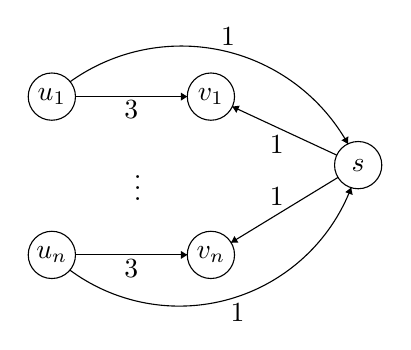
\begin{tikzpicture}[scale=0.1]
\tikzstyle{every node}+=[inner sep=0pt]
\draw [black] (18.5,-12.8) circle (3);
\draw (18.5,-12.8) node {$u_1$};
\draw [black] (38.7,-12.8) circle (3);
\draw (38.7,-12.8) node {$v_1$};
\draw [black] (18.5,-32.9) circle (3);
\draw (18.5,-32.9) node {$u_n$};
\draw [black] (38.7,-32.9) circle (3);
\draw (38.7,-32.9) node {$v_n$};
\draw (29.4,-23.4) node {$\vdots$} ;
\draw [black] (57.4,-21.5) circle (3);
\draw (57.4,-21.5) node {$s$};
\draw [black] (21.5,-12.8) -- (35.7,-12.8);
\fill [black] (35.7,-12.8) -- (34.9,-12.3) -- (34.9,-13.3);
\draw (28.6,-13.3) node [below] {$3$};
\draw [black] (21.5,-32.9) -- (35.7,-32.9);
\fill [black] (35.7,-32.9) -- (34.9,-32.4) -- (34.9,-33.4);
\draw (28.6,-33.4) node [below] {$3$};
\draw [black] (20.825,-10.907) arc (125.59934:29.18714:24.243);
\fill [black] (56.1,-18.8) -- (56.15,-17.85) -- (55.28,-18.34);
\draw (40.87,-6.38) node [above] {$1$};
\draw [black] (56.513,-24.364) arc (-20.88164:-126.45095:23.371);
\fill [black] (56.51,-24.36) -- (55.76,-24.93) -- (56.7,-25.29);
\draw (42.07,-39.01) node [below] {$1$};
\draw [black] (54.84,-23.06) -- (41.26,-31.34);
\fill [black] (41.26,-31.34) -- (42.2,-31.35) -- (41.68,-30.5);
\draw (47.05,-26.7) node [above] {$1$};
\draw [black] (54.68,-20.23) -- (41.42,-14.07);
\fill [black] (41.42,-14.07) -- (41.93,-14.86) -- (42.36,-13.95);
\draw (47.07,-17.66) node [below] {$1$};
\end{tikzpicture}
\end{center}
\end{figure}

Let us first determine the HD of $G$.
There are $2n$ shortest paths, namely $sv_i$ and $u_isv_i$ for different $i$.
We conclude that the HD is $1$, because it suffices to set $H_{v,r}=\crl{s}$ as the hitting set for every $r>0$ and $v\in V(G)$.

Now we add some costs and show that the CHD is at least $n$.
Let $c(u_iv_i)=0$ for every $i$ and set all other costs to $1$.
Note that the $1$-significant efficent paths intersecting the ball $B_s(2)$ are $u_iv_i$, which are all disjoint.
Therefore, the hitting set $H_{s,1}$ must contain at least $n$ elements.

We showed that the difference between HD and CHD is at least $n$.
We finish by noting that a similar argument shows that the sparsity of LSHS for $\calP$ is $1$, whereas the sparsity of EPHS is also lower bounded by $n$.
\end{proof}

\begin{remark}
Although this example shows the difference between HD and CHD, the reader may think that we are exploiting the maximum degree to our advantage.
This is not necessarily the case. 
In Section~\ref{app:generalhd}, where we discuss other notions of HD, we give a different, more involved, example that exhibits the same behaviour for even stronger versions of HD.
\end{remark}

It is conjectured that road networks have small HD.
Is there evidence to conjecture small CHD in these networks?
We show how doubling dimension plus an additional property, defined bellow, do imply a positive answer.
A path $P'$ \emph{partially witnesses} $P$ if $P'\subseteq P$ and $P'$ is ``long enough''.
Formally, we define the following relation for path systems.

\begin{definition}
Let $\beta\geq 0$.
We say that a path system $\calQ'$ is a $\beta$-witness of the path system $\calQ$ if, for every $Q\in\calQ$, exists $Q'\in\calQ'$ such that $Q'\subseteq Q$ and $\ell(Q')\geq 2^{-\beta}\ell(Q)$.
\end{definition}

We explore first when the system of shortest paths $\calP$ is a partial witness for the system of efficient paths $\PE$.
At an intuitive level, the partial witness property says that efficient and shortest paths are not completely different, i.e., if $Q$ is efficient, some fraction of $Q$ is shortest.
As a consequence, an important node hitting numerous paths in $\calP$, should also hit many paths in $\PE$.
The bad examples in Proposition~\ref{prop:treelike} exploit networks that do not have partial witnesses.
We stress that doubling dimension depends only on $G$ and $\ell$; the partial witness property depends on the interplay between $G$, $c$ and $\ell$.
For our result, we actually relax the partial witness property.
Notice that, in the statement of Theorem~\ref{theo:witness_doubling}, we ask only for long paths to be witnessed.

\begin{theorem}\label{theo:witness_doubling}
Assume that $G$ is $\alpha$-doubling and $\calP$ is a $\beta$-witness for $\PE_r$ for every $r\geq \frac{\log(\alpha^\beta h)}{2\log\Delta}$. \anote{There is no relation between the quantities $\alpha$ and $\Delta$ in the sense that neither bounds the other.}
If $(G,\ell)$ admits an $(h,r)$-LSHS for any $r$, then $(G,\ell,c)$ admits an $(\alpha^{\beta} h,r)$-EPHS for any $r$.
\end{theorem}
\begin{proof}
For any $r$, we need to construct a hitting set $C^E$ for $\calP_r^E$.
Assume first $r\geq \frac{\log(\alpha^\beta h)}{2\log\Delta}$.
Take $C$ as the hitting set for $\calP_{2^{-\beta}r}$, which is guaranteed to be sparse with respect to balls of radius $2^{-\beta+1}r$.
Define the desired set by
\[
C^E\defeq\{v\in C: v \text{ is in some $r$-efficient path} \}.
\]

Since $\calP$ is a $2^{-\beta}$-witness for $\PE_r$, $C^E$ is indeed a hitting set for $\PE_r$.
We are only left to prove the sparsity.
Take some $u\in V$, by doubling dimension we can cover $\Bf_{2r}(u)$ by at most $\alpha^\beta$ balls of radius $2^{-\beta+1}r$.
Each of these balls contains at most $h$ elements of $C$, therefore the sparsity is as claimed.
The argument for backward balls is identical.

Now we analyse the case $r< \frac{\log(\alpha^\beta h)}{2\log\Delta}$.
It is no longer true that the efficient paths are witnessed, but now the neigborhoods are small.
Take $C=V$ as the EPHS.
Clearly $C$ hits all the paths and the local sparsity is at most the size of the ball.
Using our assumption on $r$ and the fact that the lengths are integers, it follows that $\card{B_{2r}(v)}\leq\Delta^{2r}\leq\alpha^\beta h$. 
\end{proof}

\begin{remark}
The existence of a $\beta$-witness is not enough to bound the CHD.
Nevertheless, as discussed in Section~\ref{ssec:hldef}, the existence of $(h,r)$-LSHS already allows the construction of HL.
\end{remark}


\section{Scalable CSP Algorithms: \texorpdfstring{\\}{ } Practical Implementation}
\label{sec:numeric}

The augmented graph may contain a lot of unnecessary information.
For example, the same efficient path $uv$ can be repeated many times in the form $\pp{u,1}\pp{v,0}$, $\pp{u,2}\pp{v,1}$ and so on.
If there are not too many efficient paths, we can obtain considerable improvements both in query time and in data storage.

The idea is to construct an augmented graph without duplicated information.
The nodes are, as before, pairs $\pp{v,b}$, but an edge $(\pp{v,b},\pp{v',b'})$ is placed only if some efficient path uses it.
In other words, if we let $\calP_{s,t}^E$ be the set of all efficient paths from $s$ to $t$, we take every $P\in \calP_{s,t}^E$ with cost $b\leq B$ and trace it in the augmented graph starting at $\pp{s,b}$ and ending at $\pp{t,0}$.

\begin{definition}
The pruned augmented graph is defined by $\Gp^B=(\Vp^B,\Ep^B)$, where
\begin{align*}
\Vp^B &:=\{\pp{v,b}: v\in V, b=0,1,\ldots,B\},\\
\Ep^B &:=\{\pp{v,b}\pp{v',b'} : \exists s,t\in V, P\in\calP^E_{s,t}, c(P)\leq B, \\
&\qquad vv'\in P, b=c(P[v,t]), b'=c(P[v',t])  \}.
\end{align*}
In $\Gp^B$ all the lengths are preserved.
\end{definition}
Note that in $\Gp^B$ there are no sink nodes, hence it has at least $n$ nodes and $nB$ arcs fewer compared to $G^B$.

\subsection{HD of the pruned augmented graph}

A shortest path in $\Gp$ does not necessarily project to an efficient path, even if the path ends in a node of the form $\pp{t,0}$.
On the other hand, if $P$ projects to an efficient path, then necessarily $P$ is shortest. 
To bound the HD, the correct system to study is
\[
\tilde\calP^B:=\{P: P\text{ ends in a node }\pp{t,0}, \bar P\in \PE, c(\bar P)\leq B \}.
\]
The following result shows how the HD of this system relates to that of $\PE$.
We omit the proof since it is identical as the one in Proposition~\ref{prop:HDaugmented}.
\begin{proposition}
The HD of $\tilde\calP^B$ is $Bh_c$, where $h_c$ is the HD of $\PE$.
\end{proposition}

We use techniques described by \cite{hubimplem} together with an approach tailored for augmented graphs.
The main idea is to use contraction hierarchies first, then define the forward hub of a node as the nodes visited during a contraction-based forward search.
The backward hub is defined analogously.
These are valid hubs, since the highest rank node in a path is guaranteed to be in both hubs.

The most important parameter in CH is the rank; results vary greatly from one choice of ranks to another.
We obtain a rank in $G$ by running a greedy shortest-path cover, defined as follows.
Start with a cover $C=\varnothing$ and compute the set of all shortest paths $\calP$.
Take a node $v\notin C$ hitting most paths in $\calP$, then remove all those paths from $\calP$, add $v$ to $C$ and iterate.
The rank is defined as $n$ for the first node added to $C$, $n-1$ for the second and so on.

We work with the pruned augmented graph, i.e.\ $\tilde G_B$, which takes some time to compute, but yields considerably better hubs. 
Recall that in $\tilde G_B$ there are no sink-nodes nor ``replicated information'', since efficient paths are stored just once.
Given a rank for nodes in $G$, we contract $\tilde G_B$ as follows.
Say that $V$ is ordered according to the rank, so node $1$ is the least important and $n$ the most important.
In $\tilde G_B$, for $b=B,\ldots,0$, we contract the nodes $(1,b)$ first, then the nodes $(2,b)$ and so on till the nodes $(n,b)$ are the last to contract. 

To obtain better hubs we prune the results obtained by contraction-based searches.
If $w$ is in the forward search of $v$ with distance $d$, it might be that $\dist(v,w)<d$, this occurs because the search goes only to higher rank nodes and the discovered path is missing some node.
When $\dist(v,w)<d$, we can safely remove $w$ from the hub of $v$, since the highest ranked node in a shortest path will have the correct distance.
We describe now the process in the following steps.

\begin{enumerate}
\item Compute the shortest paths in $G$ and obtain a cover $C$
\item Compute the pruned augmented graph $\tilde G_B$
\item Contract $\tilde G_B$ using the rank given by $C$
\item Create hubs $\Lf(v),\Lb(v)$ using CH
\item Prune the hubs by running HL queries between $v$ and nodes in $\Lf(v)$. 
Run a similar process for $\Lb(v)$.
\end{enumerate}
Note that in the last step we bootstrap HL to improve it.
This works because the fact that some nodes have incorrect distance labels does not impact the correctness of a HL query; a node minimizing the distance is returned and such node must have a correct label.

%\section*{References}
\bibliographystyle{plainnat}
\bibliography{biblio}

\appendix
\section{Different notions of HD}
\label{app:generalhd}
The original definition of HD was given by \cite{highway2010}, but this is not the one we extend, but rather we work from the definition of~\cite{highway2013}.
The latter is the same as our notion except that $(i)$ we consider a less restrictive definition of path neighborhoods, that is appropriate for our needs, and $(ii)$ we generalize the notion to directed graphs and general path systems.
For $\PS$, a consequence of considering less-restrictive path-neighborhoods is that the highway dimension returned by our definition is smaller than that of \cite{highway2013}.
In particular, unlike \cite{highway2013}, the HD of $G$ as per our definition is not an upper bound to the maximum degree $\Delta$ or the doubling dimension $\alpha$.

With respect to our average HD in \cref{sec:avg_hd}, we note the following.
\begin{remark}
The algorithm in \cref{theo:preproc_avg} makes one call to the VC-dimension solver for each $C_i$.
On the other hand, the algorithm in \cite{highway2013} calls up to $n$ times the solver for each $C_i$.
Finally, there is an extra $\log n$ factor in the approximation guarantee, but now the value of $h$ can be much smaller.
\end{remark}

We now discuss how our results extend to the definition in \cite{highway2013}, which we refer to as strong-HD.
The strong-HD defines a path $P$ to be $r$-significant if, by adding at most one hop at each end, we get a shortest path $P'$ longer than $r$.
The path $P'$ is called an $r$-witness for $P$.
Intuitively, a path is significant if it represents a long path.
Observe that, if $P\in\PS$ is such that $\ell(P)>r$, then $P$ is $r$-significant by definition.
We remark also that a path can have many $r$-witnesses.

Finally, the path neighborhood must also be strengthened.
The path $P\in\PS$ belongs to $\Sf_r(v)$ if, $P$ has some $r$-witness $P'$ such that $\dist(v,P')\leq 2r$.
The reverse neighborhood $\Sb_r(v)$ is defined analogously.
With this modified versions of $r$-significant and neighborhood, the notions of LSHS and HD are the same as our previous definitions.

Under the strong-HD, we have  $\Delta\leq h$ and $\alpha\leq h+1$.
Additionally, this definition allows proving results for CH.
Finally, we show that even for the strong-HD, CHD and HD can still be off by a factor of $n$.

\begin{proposition}\label[proposition]{prop:treelike}
For any $h$, we can construct a family of networks such that the sparsity of LSHS is $h$ and that of EPHS is arbitrarily worse than $h$.
\end{proposition}
\begin{proof}
First, we construct an example where the sparsity grows from $h$ to $h^2$.
Consider an $h$-ary tree rooted at $u$ with three levels, i.e., with $1+h+h^2$ nodes.
Now add a node $v$ with $h$ children as in Figure~\ref{fig:treelike}. 
The grandchildren of $v$ are the same as the grandchildren of $u$.

All the edges are bidirectional and have unit cost.
The lengths are as follows: $ux_i$ and $vy_i$ (dashed in Figure~\ref{fig:treelike}) are zero; $uv$ and from $y_i$ to the leafs is one; from $x_i$ to the leafs is three.
It is easy to see that the sparsity of a LSHS is $h+1$.

On the other hand, every leaf $w$ is a $2$-efficient path.
Indeed, it can be extended to $x_iw$ that is the shortest path from $x_i$ to $w$ with constraint 1.
All the leafs are in the ball $B_4(u)$, so the sparsity is at least $h^2$.

\begin{figure}
\centering
\includegraphics[scale=0.5]{TexImg/Treelike.pdf}
\caption{Example where the EPHS is much larger than the LSHS.}\label{fig:treelike}
\end{figure}

The general case works in the same fashion.
We make the sparsity grow to $h^k$ by creating two complete, $k$-level, $h$-ary trees $T$ and $T'$.
Connect the root of $T$ to the root of $T'$ and the leafs of both trees are shared.
Observe that the number of nodes is 
\begin{align*}
n &=[\text{$k$-level $h$-ary tree}] + [\text{$(k-1)$-level $h$-ary tree}]\\
&= ({h^{k+1}-1})/({h-1}) + ({h^k-1})/({h-1}),
\end{align*}
therefore the sparsity is $\Theta(n)$, the worst possible.
\end{proof}

\section{Contraction Hierarchies}
\label{sec:ch}
We present here how to extend the concept of HD in order to prove the efficiency of CH in directed graphs.
Given a rank in the nodes, the shortcut process works as in the non-directed case:
\begin{enumerate}
	\item Let $G'$ be a temporary copy of $G$.
	\item Remove nodes of $G'$ and its edges in increasing rank.
	\item When removing $v$, if some unique shortest path in $G$ uses $uvw$, add $(u,w)$ to $G'$ with length $\ell(u,v)+\ell(v,w)$.
\end{enumerate}

Call $E^+$ the set of edges created in the shortcut process.
A source-destination query runs bidirectional Dijkstra, but each search only considers paths of increasing ranks.

As in the non-directed case, let $Q_i=C_i\setminus \cup_{j>i}C_j$ be the partition of $V$.
All the ranks in $Q_i$ are smaller than those in $Q_{i+1}$, within each $Q_i$ the rank is arbitrary.

\begin{lemma}\label{lemma:intshort}
	Let $P$ be a shortest path in the original graph.
	If $P$ has at least three vertices and $\ell(P)>2^{\gamma}$, then some internal vertex of $P$ belongs to a level $Q_x$, $x>\gamma$.
\end{lemma}
\begin{proof}
	The path $P'$ obtained by removing the endpoints of $P$ is $\ell(P)$-significant.
	By definition of the $C_i$'s, $C_{\gamma+1}$ hits $P'$ at some node $u$.
	By construction of the partition, $u\in Q_x$ with some $x>\gamma$. 
\end{proof}

Now we show that each node adds at most $h$ to its out-degree for each $Q_i$, so the process adds at most $h\log D$ to the out-degree of each node.
\begin{lemma}
	Assume the network admits the $C_i$'s.
	For any $v$ and fixed $j$, the number of shortcuts $(v,w)$ with $w\in Q_j$ is at most $h$.
\end{lemma}
\begin{proof}
	Let $i$ be the level such that $v\in Q_i$ and define $\gamma:=\min(i,j)$.
	We claim that $w\in \Bf_{2^\gamma}(v)$.
	Assume the claim, then the number of shortcuts is at most $\card{Q_j\cap \Bf_{2^\gamma}(v)}$, but using local sparsity and set inclusion:
	\[
	\card{Q_j\cap \Bf_{2^\gamma}(v)}\leq \card{C_j\cap\Bf_{2\cdot 2^{j-1}}(v)} \leq h.
	\]
	
	All that remains is to prove the claim.
	The shortcut $(v,w)$ was created when the process removed the last internal vertex of the shortest path $P(v,w)$ in $G$.
	Necessarily all the internal vertices are in levels at most $\gamma$, because they were removed before $v$ and $w$, hence they have lower rank.
	Finally, apply Lemma~\ref{lemma:intshort} to conclude that $\ell(P(v,w))\leq 2^\gamma$.
\end{proof}

We need to bound the in-degree, because it could be that some node $v$ is receiving many edges.
The proof is basically the same.
\begin{lemma}
	Assume the network admits the $C_i$'s.
	For any $v$ and fixed $j$, the number of shortcuts $(w,v)$ with $w\in Q_j$ is at most $h$.
\end{lemma}
\begin{proof}
	Same as in the previous lemma, but now $w\in \Bb_{2^\gamma}(v)$.
\end{proof}

We can conclude now that the number of shortcuts, i.e.\ $\card{E^+}$, is at most $2nh\log D$.

As we mentioned before, the query performs Dijkstra from the source and target, but always constructing paths of increasing rank.
When scanning a vertex $v$, the forward search has a label $\dist(s,v)'$. 
The labels always satisfy $\dist(s,v)'\geq\dist(s,v)$, but, since the algorithm only goes to higher ranks, equality is not guaranteed.

We add a pruning rule analogous to the non-directed case: when the forward search scans a node $v$, if $(v,w)\in E\cup E^+$ and $w\in Q_i$, then $w$ is added to the priority queue only if $\text{rank}(w)>\text{rank}(v)$ and $\dist(s,v)'+\ell(v,w)\leq 2^i$.
For the reverse search, the condition is the analogous $\dist(v,t)'+\ell(w,v)\leq 2^i$ when $(w,v)\in  E\cup E^+$.

\begin{proposition}
	The query with additional pruning returns the correct distance.
	Additionally, each Dijkstra scans at most $h$ nodes in each level.
\end{proposition}
\begin{proof}
	Let us analyse the forward search.
	Say the node $v$ is being scanned, $w\in Q_i$ is a candidate and $\dist(s,v)'+\ell(v,w)>2^i$.
	If the current path $P'$ to $w$ is optimal, then $P(s,w)$ is $2^i$-significant and it is hit by $C_{i+1}$. 
	As a consequence, $P(s,w)$ contains an internal vertex with higher rank than $w$.
	This vertex cannot be in $P'$ nor a shortcut containing it, thus contradicting the optimality of $P'$.
	We conclude that $P'$ is not optimal and $w$ can be ignored.
	
	Bounding the number of scanned nodes is easy; every $w\in Q_i$ added to the queue satisfies $w\in \Bf_{2^i}(s)$, so applying local sparsity we finish the proof.
\end{proof}

As a result, the forward search adds at most $h\log D$ nodes to the queue;
each of node amounts to $O(\text{outdeg} (G^+))$ operations, i.e., $O(\text{outdeg}(G) + h\log D)$ operations.


\section{CHD vs. HD: Extensions}
\label{app:extn}
\input{sec_extensions.tex}


\section{Additional Proofs}
\label{sec:proofs}
\begin{proofof}{Proposition~\ref{prop:poly_lshs}}
Denote $S_r(v):=\Sf_r(v,\calQ)\cup\Sb_r(v,\calQ)$. 
Observe that, for fixed $v\in V$, the set system $(E,\{\pi(Q):Q \in S_r(v)\})$ admits a hitting set of size $h\Delta$.
Indeed, we know that exists $H_{v,r}\subseteq V$, $\card{H_{v,r}}\leq h$, hitting every path in $\Sf_r(v,\calQ)$ and in $\Sb_r(v,\calQ)$.
The desired hitting set consists of all the edges adjacent to a node in $H_{v,r}$.

If the minimum size of a set system is $s$ and the VC-dimension is $d$, then the algorithm in \cite{vc_dim_hitting} obtains, in polynomial time, a hitting set of size at most $\Or(sd\log(sd))$.
In particular, we can use the algorithm to obtain a set $\tilde F_{v,r}\subseteq E$, of size at most $h'=\Or(h\Delta\log(h\Delta))$, hitting the set system $(E,\{\pi(Q):Q \in S_r(v)\})$ .

Consider the set $F_{v,r}\subseteq V$ that contains all the endpoints of edges in $\tilde F_{v,r}$.
It follows that $F_{v,r}\subseteq V$ can be obtained in polynomial time and is a hitting set for $S_r(v)$ of size $\card{F_{v,r}}\leq 2h'$.

Assume for now that we know the value of $h$.
Note that the value $h'$ can be computed from $h$ and the guarantee given by the oracle, i.e., the constant inside the big-O.
We construct the $(2h',r)$-LSHS iteratively.
At each iteration $i$ we maintain the following invariant: $C_i$ hits every path in $\calQ_r$.
In an iteration we check if $C_i$ is locally sparse, if not, we strictly reduce the cardinality of $C_i$ while maintaining the invariant.
Start with $C_0=V$. 
Let $B_{2r}(v):=\Bf_{2r}(v)\cup \Bb_{2r}(v)$.
Assume $v\in V$ is such that $\card{B_{2r}(v)\cap C_i}>2h'$ and let $C_{i+1}:=(C_i\setminus B_{2r}(v))\cup F_{v,r} $.
The cardinality strictly decreases and we only need to check the invariant.
Consider the paths hit by nodes removed in $C_i$, this set is
\begin{align*}
&\hspace{-1cm}\{Q\in\calQ_r: Q\cap C_i\cap B_{2r}(v)\neq \varnothing\}\\
&\subseteq \{Q\in\calQ_r: Q\cap B_{2r}(v)\neq \varnothing\} \subseteq S_r(v).
\end{align*}
Since $F_{v,r}$ hits $S_r(v)$, the proof is completed.

If we do not know the value of $h$, we can do a doubling search for $h'$. 
Indeed, if the guess of $h'$ is low, then at some point it could be that $\card{F_{v,r}}>2h'$, then we double $h'$ and restart the process.
\end{proofof}






\end{document}
